% !TeX program = xelatex
\documentclass[a4paper,fontsize=10.2pt,parskip=half-]{scrartcl}
\usepackage[a4paper,left=2.45cm,right=2.45cm,top=2.3cm,bottom=2.4cm,footskip=1.1cm]{geometry}
\usepackage{fontspec}
\setmainfont{TeX Gyre Pagella}[Numbers={Lining,Proportional}]
\setsansfont{Inter}[Scale=0.88,BoldFont={Inter SemiBold},Numbers={Lining},RawFeature={-calt}]
\newfontfamily\tabfont{Inter}[Scale=0.80,BoldFont={Inter SemiBold},Numbers={Lining,Tabular},RawFeature={-calt}]
\usepackage[none]{hyphenat}
\usepackage{graphicx,booktabs,array,tabularx,enumitem,caption,float,xcolor}
\usepackage[hidelinks,pdflang={en-US},urlbordercolor={0 0 0},linkbordercolor={0 0 0},citebordercolor={0 0 0},pdftitle={Hedging the Dollar at Four Percent},pdfauthor={Mergim Manxholli},pdfsubject={Independent analysis based on public information as of 11 November 2026. Not investment advice.}]{hyperref}
\usepackage{scrlayer-scrpage}
\newcommand{\NMonths}{327}
\newcommand{\SpotStart}{1.4925}
\newcommand{\SpotEnd}{0.8230}
\newcommand{\SpotFall}{44.9}
\newcommand{\SpotPa}{2.2}
\newcommand{\CarryCum}{38.9}
\newcommand{\CarryPa}{1.8}
\newcommand{\AvgDiff}{1.8}
\newcommand{\RetLocal}{8.6}
\newcommand{\RetU}{6.2}
\newcommand{\RetH}{6.3}
\newcommand{\RetGap}{0.1}
\newcommand{\VolU}{16.3}
\newcommand{\VolH}{15.1}
\newcommand{\VolStar}{14.8}
\newcommand{\DDU}{62.2}
\newcommand{\DDH}{52.4}
\newcommand{\WorstU}{40.6}
\newcommand{\WorstH}{44.8}
\newcommand{\GrowthU}{516}
\newcommand{\GrowthH}{531}
\newcommand{\HStar}{70}
\newcommand{\HStarLo}{48}
\newcommand{\HStarHi}{92}
\newcommand{\HStarSE}{0.11}
\newcommand{\HStarDec}{0.70}
\newcommand{\CorrAbs}{0.18}
\newcommand{\VolFx}{9.6}
\newcommand{\XMeanAbs}{0.1}
\newcommand{\XSE}{1.8}
\newcommand{\XT}{0.05}
\newcommand{\ShareMonths}{50.8}
\newcommand{\YearsHedgedBeats}{14}
\newcommand{\FullYears}{26}
\newcommand{\RetHCostA}{6.1}
\newcommand{\RetHCostB}{5.8}
\newcommand{\BreakEvenCost}{0.11}
\newcommand{\HTwo}{44}
\newcommand{\HThree}{37}
\newcommand{\RollHLast}{34}
\newcommand{\WUp}{11}
\newcommand{\WDown}{9}
\newcommand{\WAvgFx}{1.5}
\newcommand{\IUS}{3.94}
\newcommand{\DiffNow}{3.98}
\newcommand{\CarryNow}{3.9}
\newcommand{\Pctile}{95}
\newcommand{\BreakEvenSpot}{0.791}
\newcommand{\CalLocal}{17.9}
\newcommand{\CalFxAbs}{12.5}
\newcommand{\CalU}{3.2}
\newcommand{\CalH}{13.3}
\newcommand{\YtdU}{15.9}
\newcommand{\YtdH}{7.7}
\newcommand{\EarlyLocalAbs}{7.5}
\newcommand{\EarlyFxAbs}{9.5}
\newcommand{\EarlyUAbs}{16.3}
\newcommand{\EarlyHAbs}{8.3}
\newcommand{\DDHCostB}{53.4}
\newcommand{\GrowthHCostB}{464}
\newcommand{\WorstHFx}{11.9}
\newcommand{\RegUTwo}{4.39}
\newcommand{\RegTqTwo}{0.64}
\newcommand{\RegEightyTwo}{0.57}
\newcommand{\RegHTwo}{1.35}
\newcommand{\BlockMonths}{109}
\newcommand{\TerHighX}{2.8}
\newcommand{\TerHighT}{1.0}
\newcommand{\TerHighSpotAbs}{0.7}
\newcommand{\TerHighCarryAbs}{3.6}
\newcommand{\TerLowXAbs}{3.2}
\newcommand{\FamaBetaAbs}{0.70}
\newcommand{\FamaSE}{1.17}
\newcommand{\MinimaxH}{80}
\newcommand{\AltTwo}{70}
\newcommand{\AltFour}{80}
\newcommand{\AltFive}{75}
\newcommand{\CashCall}{23}
\newcommand{\FillRate}{0.76}

\makeatletter\newcommand{\tabinput}[1]{\@@input #1 }\makeatother

\color{black}
\raggedright
\setlength{\parindent}{0pt}
\linespread{1.06}
\setkomafont{section}{\sffamily\bfseries\fontsize{12.5}{15}\selectfont}
\setkomafont{subsection}{\sffamily\bfseries\normalsize}
\RedeclareSectionCommand[beforeskip=1.1em,afterskip=0.35em]{section}
\captionsetup{font={sf,small},labelfont=bf,labelsep=period,justification=raggedright,singlelinecheck=false,skip=4pt}
\setlist{leftmargin=1.5em,itemsep=0.25em,topsep=0.3em,parsep=0pt}
\newlist{assume}{itemize}{1}
\setlist[assume]{leftmargin=2.2em,labelwidth=1.6em,labelsep=0.6em,align=left,itemsep=0.25em,topsep=0.3em,parsep=0pt}
\clearpairofpagestyles
\cfoot{\sffamily\scriptsize Mergim Manxholli \textbar{} Hedging the Dollar at Four Percent \textbar{} November 2026 \textbar{} Not investment advice \hfill \thepage}
\setkomafont{pagefoot}{\normalfont}
\newcommand{\src}[1]{\par\vspace{2pt}{\sffamily\fontsize{7.2}{9.2}\selectfont #1\par}}
\newcolumntype{L}[1]{>{\raggedright\arraybackslash}p{#1}}
\newcolumntype{Y}{>{\raggedright\arraybackslash}X}
\newcommand{\lead}[1]{\textbf{#1}}
\renewcommand{\arraystretch}{1.18}
\urlstyle{same}

\begin{document}

% ------------------------------------------------------------------ cover
\begin{titlepage}
\raggedright
\vspace*{2.2cm}
{\sffamily\small\bfseries RESEARCH NOTE \textbar{} CURRENCY HEDGING FOR SWISS FRANC INVESTORS\par}
\vspace{0.9cm}
\rule{\textwidth}{1.2pt}\par
\vspace{0.9cm}
{\sffamily\bfseries\fontsize{30}{35}\selectfont Hedging the Dollar\\ at Four Percent\par}
\vspace{0.9cm}
{\fontsize{14}{19}\selectfont\itshape How much of its US equity exposure should a Swiss franc investor hedge? Evidence from \NMonths{} months of public data, August 1999 to October 2026.\par}
\vspace{0.9cm}
\rule{\textwidth}{0.4pt}\par
\vfill
{\sffamily\bfseries\Large Mergim Manxholli\par}
\vspace{0.25cm}
{\sffamily\large November 2026\par}
\vspace{1.0cm}
{\sffamily\small Independent analysis based on public information as of 11 November 2026. Not investment advice.\par}
\vspace*{0.6cm}
\end{titlepage}

% ------------------------------------------------------------------ summary
\addsec{Summary}

\lead{The question.} In September 2026 three month dollar rates averaged \IUS\% and three month franc rates stood just below zero. A Swiss franc investor who hedges dollar assets gives up the carry that this rate gap implies, about \CarryNow\% a year. The gap has been narrower in \Pctile\% of months since July 1999. A common argument is that hedging US equities has therefore become too expensive. This note tests that argument on \NMonths{} months of public data for the S\&P 500.

\lead{The answer.} Hedge about three quarters of the exposure, and do not let the carry drive the decision. Four findings support this.

\begin{enumerate}[label=\textbf{\arabic*.}]
\item \lead{The carry has not been a cost.} From August 1999 to October 2026 a fully hedged S\&P 500 position returned \RetH\% a year in francs and an unhedged one \RetU\%. The dollar fell \SpotPa\% a year against the franc, slightly more than the \CarryPa\% a year that the rate gap had charged hedgers. The difference between the two strategies is not statistically different from zero.
\item \lead{Volatility is lowest at a hedge ratio of about \HStar\%, not 100\%.} Volatility falls from \VolU\% unhedged to \VolStar\% at a ratio of \HStar\% and rises back to \VolH\% fully hedged, because the dollar has tended to move against US equities: on average it gained against the franc in months when the S\&P 500 fell and lost in months when it rose. The 95\% confidence interval for the best ratio runs from \HStarLo\% to \HStarHi\%.
\item \lead{The best ratio moves with the regime, and the two possible errors are not equally costly.} It was above 100\% before September 2008 and near 40\% afterward. In each of three consecutive periods of \BlockMonths{} months a ratio of 75\% stayed within \RegTqTwo{} volatility points of the best ratio between 0\% and 100\%, and a ratio of 80\% within \RegEightyTwo. An unhedged position was up to \RegUTwo{} points worse and a fully hedged one up to \RegHTwo.
\item \lead{A rate gap of four points is a weak signal.} In the third of months with the widest gap the dollar fell by less than the forward implied, and unhedged positions did better by \TerHighX\% a year. The t~statistic of that result is \TerHighT. That is not enough evidence to move a strategic ratio.
\end{enumerate}

Table 1 gives the full picture by hedge ratio.

\begin{table}[H]
\caption{US equities in Swiss francs by hedge ratio, August 1999 to October 2026}
{\tabfont
\begin{tabularx}{\textwidth}{@{}X r r r r r r@{}}
\toprule
Hedge ratio & Return & Volatility & Maximum & Worst 12 & Sharpe & CHF 100 \\
 & \% a year & \% a year & drawdown \% & months \% & ratio & grows to \\
\midrule
\tabinput{t1.tex}
\bottomrule
\end{tabularx}}
\src{S\&P 500 Total Return Index converted to francs. Month end data, \NMonths{} months. Sharpe ratio against the Swiss three month rate. Hedging by rolling one month forwards priced from the rate gap (assumptions A1 to A4, section 1). Sources: Yahoo Finance, Federal Reserve H.10, OECD via FRED; own calculations.}
\end{table}

\lead{What this means for a portfolio.} For a Swiss institution the strategic hedge ratio on US equities belongs between 70\% and 80\%. The usual alternatives, fully hedged because foreign currency is uncompensated risk, or unhedged because the hedge costs four percent, are both weaker on the evidence. The note also shows what would change this view: the hedge ratio that minimized volatility over the latest five years is only \RollHLast\%, and an investor who believes that pattern is permanent can defend a ratio well below three quarters. The case against that belief is set out in section 4.

% ------------------------------------------------------------------ 1
\clearpage
\section{Data and method}

Everything in this note can be reproduced from three public sources. The data files and scripts are available on request.

\begin{table}[H]
\caption*{\textbf{Inputs.} Three public sources}
{\tabfont
\begin{tabularx}{\textwidth}{@{}L{2.4cm} Y L{6.2cm}@{}}
\toprule
Input & Definition & Source and date \\
\midrule
US equities & S\&P 500 Total Return Index in dollars, last close of each month, July 1999 to October 2026 & Yahoo Finance, ticker \textasciicircum SP500TR, retrieved 11~November~2026 \\
Exchange rate & Swiss francs per US dollar, noon buying rate in New York, last observation of each month & Federal Reserve Board, H.10 release, FRED series DEXSZUS, updated 9 November 2026 \\
Interest rates & Three month interbank rates for Switzerland and the United States, monthly averages, percent a year & OECD Main Economic Indicators via FRED, series IR3TIB01CHM156N and IR3TIB01USM156N, updated 15 October 2026 \\
\bottomrule
\end{tabularx}}
\end{table}

\lead{Sample.} The Swiss rate series starts in July 1999, which sets the start of the sample. The first monthly return is August 1999 and the last is October 2026, which gives \NMonths{} months.

\lead{Terms.} The rate gap is the three month dollar rate minus the three month franc rate. The forward discount is the fall of the dollar that this gap builds into a forward contract. The carry is what the hedger gives up by selling dollars at that discount.

\lead{Returns.} With P the index level, S the franc price of one dollar, i the annual interest rate written as a decimal, and subscripts 0 and 1 for the start and end of a month:

{\sffamily\small
\begin{tabular}{@{}ll@{}}
Unhedged return in francs & R\textsubscript{U} = (P\textsubscript{1} / P\textsubscript{0}) × (S\textsubscript{1} / S\textsubscript{0}) − 1 \\
One month forward rate & F\textsubscript{0} = S\textsubscript{0} × (1 + i\textsubscript{CHF} / 12) / (1 + i\textsubscript{USD} / 12) \\
Return with hedge ratio h & R\textsubscript{h} = R\textsubscript{U} − h × (S\textsubscript{1} − F\textsubscript{0}) / S\textsubscript{0} \\
Ratio that minimizes volatility & h* = Cov(R\textsubscript{U}, X) / Var(X), with X = (S\textsubscript{1} − F\textsubscript{0}) / S\textsubscript{0} \\
\end{tabular}}

The investor sells forward, for one month, a share h of the dollar value held at the start of the month and repeats this every month. Gains and losses on equities during the month stay unhedged, as they would in practice.

\lead{Assumptions.} These are modeling choices, not data.

\begin{assume}
\item[\textbf{A1}] This note found no free public source of one month forward rates for the full period. Forward rates are therefore rebuilt from covered interest parity using the two OECD rate series. Du, Tepper and Verdelhan (2018) show that after the 2008 crisis the franc traded with a persistent negative basis against the dollar, of more than 20 basis points on average at the three month horizon from 2010 to 2016, which makes real hedges somewhat more expensive than this proxy. The two OECD series also share one definition but may rest on different instruments in the two countries. Section 2 therefore reports results with an extra cost of 0.25 and 0.50 points a year.
\item[\textbf{A2}] The monthly average three month rate stands in for the one month rate at the end of that month.
\item[\textbf{A3}] The US rate for April 2020 is missing in the source. It is set to \FillRate\%, the average of March and May 2020.
\item[\textbf{A4}] No transaction costs, taxes or collateral costs. The index is gross of dividend withholding tax.
\end{assume}

% ------------------------------------------------------------------ 2
\section{The carry has not been a cost}

At the end of July 1999 one dollar cost \SpotStart{} francs. At the end of October 2026 it cost \SpotEnd. That is a fall of \SpotFall\%, or \SpotPa\% a year. Over the same period the rate gap averaged \AvgDiff{} points, and an investor who sold dollars forward every month locked in a cumulative depreciation of \CarryCum\%, or \CarryPa\% a year. The forward market charged hedgers for a fall in the dollar, and the dollar then fell by a little more than that (figure 1).

\begin{figure}[H]
\caption{The dollar fell slightly more than the rate gap implied}
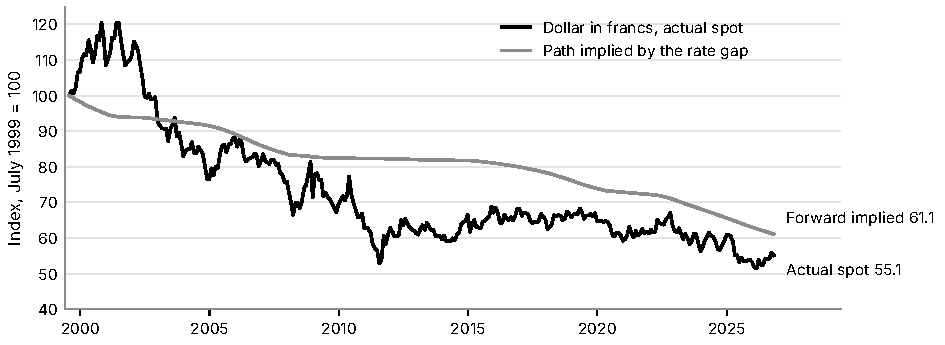
\includegraphics[width=\textwidth]{../out/fig1_spot_vs_forward.pdf}
\src{Dollar in francs, July 1999 = 100. The gray line compounds the one month forward discount implied by the rate gap. Sources: Federal Reserve H.10, OECD via FRED; own calculations.}
\end{figure}

The two strategies therefore earned almost the same (figure 2). CHF 100 invested in July 1999 grew to CHF \GrowthH{} fully hedged and CHF \GrowthU{} unhedged, against a return of \RetLocal\% a year for the index in dollars. Before compounding, staying unhedged earned \XMeanAbs{} point a year more than hedging, with a simple t~statistic of \XT. The standard error of that average is \XSE{} points a year, so the test has little power: the data reject neither a zero cost nor a cost as large as the average rate gap of \AvgDiff{} points a year. After compounding the hedged position ends \RetGap{} point a year ahead because it was less volatile. Unhedged beat hedged in \ShareMonths\% of months. Hedged beat unhedged in \YearsHedgedBeats{} of the \FullYears{} full calendar years from 2000 to 2025.

\begin{figure}[H]
\caption{CHF 100 invested in the S\&P 500 in July 1999}
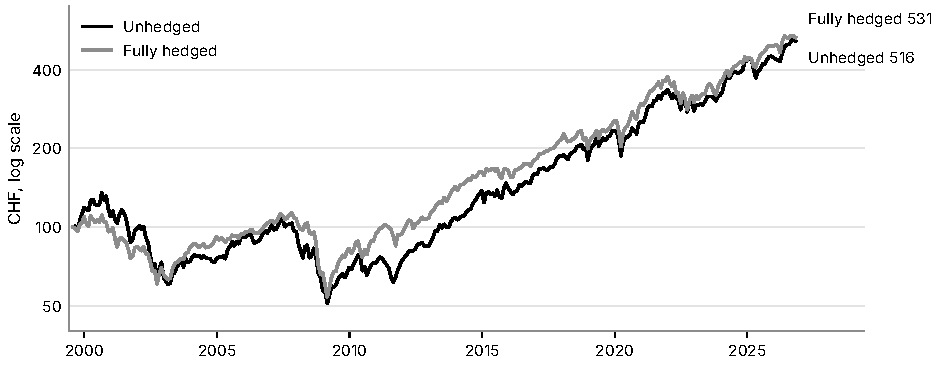
\includegraphics[width=\textwidth]{../out/fig2_growth.pdf}
\src{Month end values, dividends reinvested. Sources: Yahoo Finance, Federal Reserve H.10, OECD via FRED; own calculations.}
\end{figure}

\lead{Sensitivity to the forward proxy.} An extra hedging cost of 0.25 points a year lowers the fully hedged return to \RetHCostA\% and an extra 0.50 points lowers it to \RetHCostB\%, which would leave CHF \GrowthHCostB{} at the end. The two strategies tie at an extra cost of \BreakEvenCost{} points a year. The fair reading is that returns were a draw within the precision of the proxy. A constant extra cost leaves volatility and the hedge ratio unchanged, and moves the maximum drawdown of the hedged position by one point (from \DDH\% to \DDHCostB\% with 0.50 points). A basis that widens in a crisis, as opposed to a constant cost, is not captured. The decision therefore has to be made on risk.

% ------------------------------------------------------------------ 3
\section{Volatility is lowest at about 70\% hedged}

If currency moves were unrelated to equity returns, a full hedge would remove a source of risk and the best ratio would be 100\%. For the dollar and the franc that is not what the data show. Over the full sample the correlation between monthly S\&P 500 returns in dollars and the change in the dollar against the franc is minus \CorrAbs. The dollar, with an annual volatility of \VolFx\% against the franc, has been a partial cushion for a Swiss holder of US equities.

The ratio that minimizes volatility is the slope of a regression of the unhedged return on the currency payoff X. It is \HStarDec, with a Newey West standard error of \HStarSE{} (six lags), so the 95\% interval runs from \HStarLo\% to \HStarHi\%. Both zero and 100\% lie outside it. Figure 3 shows how flat the curve is around the minimum: any ratio from 50\% to 90\% gives volatility within 0.2 points of the lowest value, \VolStar\%.

Volatility is not the only measure of risk. The maximum drawdown falls as the hedge ratio rises, from \DDU\% unhedged to \DDH\% fully hedged, and is flat above a ratio of 90\%. The worst twelve months, by contrast, were worse for the hedged investor (\WorstH\% against \WorstU\%): the hedged position's worst window, March 2008 to February 2009, was one in which the dollar rose \WorstHFx\% against the franc.

\begin{figure}[H]
\caption{Volatility by hedge ratio, full sample and three consecutive periods}
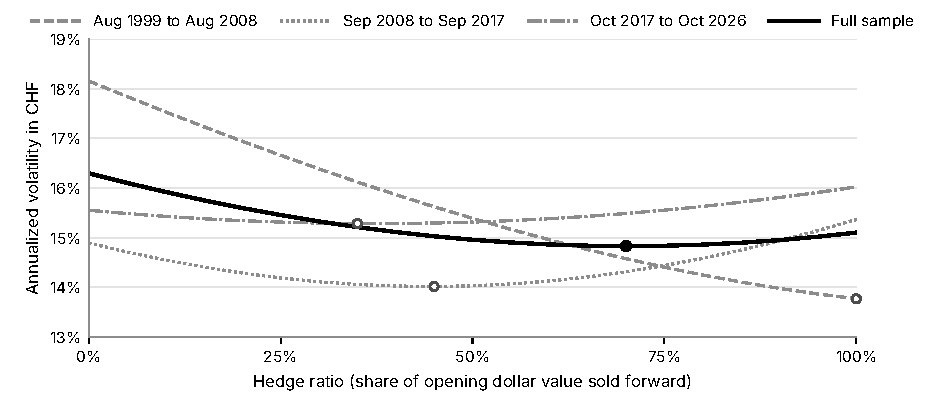
\includegraphics[width=\textwidth]{../out/fig3_vol_vs_hedge.pdf}
\src{Annualized standard deviation of monthly returns in francs. Dots mark the lowest point of each curve between 0\% and 100\%. Sources: Yahoo Finance, Federal Reserve H.10, OECD via FRED; own calculations.}
\end{figure}

% ------------------------------------------------------------------ 4
\section{The best ratio moves with the regime}

The full sample hides two different worlds. Splitting the \NMonths{} months into three equal blocks of \BlockMonths{} months, with no attempt to pick the break dates, gives table 2.

\begin{table}[H]
\caption{Three consecutive periods of \BlockMonths{} months}
{\tabfont
\begin{tabularx}{\textwidth}{@{}X r r r r r r r r@{}}
\toprule
 & \multicolumn{2}{c}{Return \% a year} & \multicolumn{2}{c}{Volatility \% a year} & Correl. & Best & Dollar & Rate \\
Period & Unhedged & Hedged & Unhedged & Hedged & & ratio & \% a year & gap \\
\midrule
\tabinput{t2.tex}
\bottomrule
\end{tabularx}}
\src{Correl. is the correlation between S\&P 500 returns in dollars and the change in the dollar against the franc. Best ratio minimizes volatility within the period, with no cap at 100\%. Rate gap is the average dollar rate minus franc rate in points. Own calculations from the sources in section 1.}
\end{table}

Until August 2008 the dollar tended to fall with US equities. A full hedge cut volatility by more than four points and the best ratio was above 100\%. Since September 2008 the dollar has tended to rise when US equities fall, the best ratio has been \HTwo\% and then \HThree\%, and a fully hedged position has been slightly more volatile than an unhedged one. Figure 4 shows the same shift on rolling five year windows. One plausible reading, which this note does not test, is that since 2008 demand for dollars in periods of stress has outweighed the safe haven status of the franc.

\begin{figure}[H]
\caption{Rolling five year view of the equity and currency relationship}
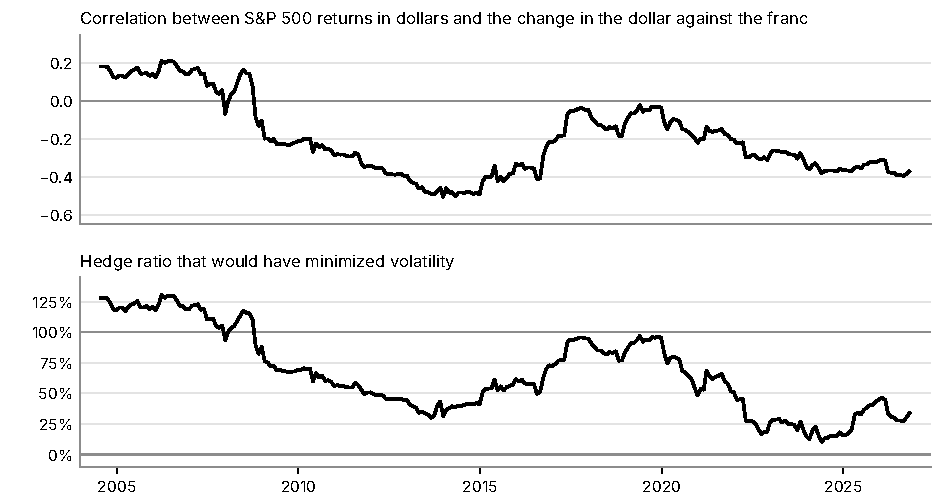
\includegraphics[width=\textwidth]{../out/fig4_rolling.pdf}
\src{Windows of 60 months, plotted at the end of each window. Latest window: November 2021 to October 2026. Sources: Yahoo Finance, Federal Reserve H.10, OECD via FRED; own calculations.}
\end{figure}

\lead{The cushion is real but unreliable.} In the 20 worst months for the S\&P 500 the dollar rose against the franc \WUp{} times and fell \WDown{} times, with an average gain of \WAvgFx\%. Table 3 lists every fall of at least 15\% in the S\&P 500 on month end data and adds the first months of 2025.

\begin{table}[H]
\caption{Equity drawdowns: what the dollar did, and what the investor got}
{\tabfont
\begin{tabularx}{\textwidth}{@{}X r r r r@{}}
\toprule
 & S\&P 500 & Dollar against & Unhedged & Fully hedged \\
Month end to month end & in USD \% & the franc \% & in CHF \% & in CHF \% \\
\midrule
\tabinput{t3.tex}
\bottomrule
\end{tabularx}}
\src{The first five rows are all the falls of at least 15\% in the S\&P 500 in dollars from a month end peak to the following trough, where a trough is the lowest month end before a recovery of at least 15\%. The memo row is below that threshold: it runs from the month end high of January 2025 to the low of April 2025. Own calculations from the sources in section 1.}
\end{table}

The dollar helped in 2011 and 2022, did nothing in 2008 and 2020 taken as whole episodes, and hurt badly in 2000 to 2002. In early 2025 it again fell together with equities: from the end of January to the end of April the S\&P 500 lost \EarlyLocalAbs\% in dollars, the dollar lost \EarlyFxAbs\% against the franc, and an unhedged Swiss investor lost \EarlyUAbs\% against \EarlyHAbs\% for a hedged one. Over calendar 2025 as a whole the index gained \CalLocal\% in dollars, but the dollar fell \CalFxAbs\%, leaving \CalU\% unhedged against \CalH\% hedged. In the first ten months of 2026 the order reversed, with \YtdU\% unhedged against \YtdH\% hedged.

\lead{Choosing a ratio when the regime is unknown.} A ratio does not have to be the best in any one regime. It has to avoid being far from the best in every regime. Table 4 measures that directly.

\begin{table}[H]
\caption{Volatility in each period and the worst shortfall against the best ratio}
{\tabfont
\begin{tabularx}{\textwidth}{@{}X r r r r@{}}
\toprule
 & Aug 1999 to & Sep 2008 to & Oct 2017 to & Worst shortfall, \\
Hedge ratio & Aug 2008 & Sep 2017 & Oct 2026 & points \\
\midrule
\tabinput{t4.tex}
\bottomrule
\end{tabularx}}
\src{Annualized volatility in percent. Ratios from 0\% to 100\% in steps of five points. The best ratio is the one with the lowest volatility on that grid. Shortfalls are computed from unrounded figures, so they can differ by 0.01 from the rounded values shown. Own calculations from the sources in section 1.}
\end{table}

The ratio with the smallest worst case is \MinimaxH\%, and 75\% is almost as good. The result does not hinge on the choice of three blocks: with two, four or five nearly equal blocks the ratio with the smallest worst case is \AltTwo\%, \AltFour\% and \AltFive\%. The asymmetry is the central point: hedging too little cost up to \RegUTwo{} points of volatility, and hedging too much cost up to \RegHTwo. An investor who is unsure which regime comes next should lean toward the higher end of the plausible range. That is why this note recommends about three quarters, and not the \RollHLast\% that the latest five years alone would suggest.

% ------------------------------------------------------------------ 5
\section{Is four percent a reason to hedge less?}

The rate gap was \DiffNow{} points in September 2026 (figure 5). Compounded over twelve months it implies a forward discount of \CarryNow\%. With the dollar at \SpotEnd{} francs on 30 October 2026, a one year hedge struck at these rates breaks even if the dollar is at about \BreakEvenSpot{} francs a year later. Above that level the unhedged investor wins. These are proxy values from assumption A1, not market quotes.

\begin{figure}[H]
\caption{Rate gap: three month dollar rate minus three month franc rate}
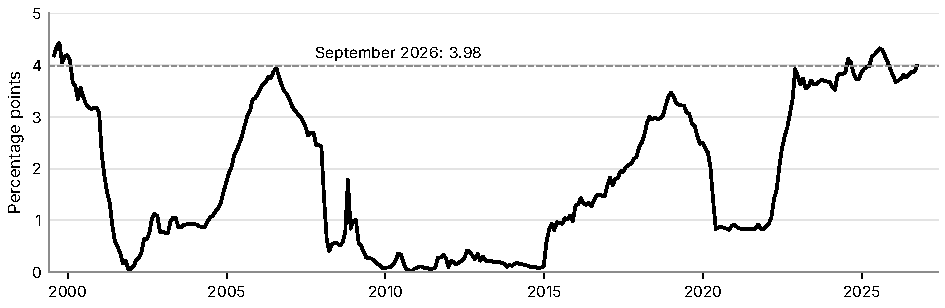
\includegraphics[width=\textwidth]{../out/fig5_rate_gap.pdf}
\src{Monthly averages, July 1999 to September 2026. The US value for April 2020 is interpolated (A3). Source: OECD Main Economic Indicators via FRED; own calculations.}
\end{figure}

Section 2 showed that over the full sample the forward was close to a fair price. The more useful question is whether that still holds when the gap is wide. Table 5 sorts all months into three equal groups by the rate gap known at the start of the month.

\begin{table}[H]
\caption{What followed narrow, middle and wide rate gaps}
{\tabfont
\begin{tabularx}{\textwidth}{@{}X r r r r r r@{}}
\toprule
Rate gap at start & Range, & Months & Dollar change & Change implied by & Unhedged minus & t statistic \\
of month & points & & \% a year & the forward \% a year & hedged \% a year & \\
\midrule
\tabinput{t5.tex}
\bottomrule
\end{tabularx}}
\src{Arithmetic averages of monthly figures multiplied by twelve. Simple t statistics (mean over its standard error). The last return column is computed from unrounded figures. The three groups are thirds of the full sample, so the cut points use information from the whole period. Own calculations from the sources in section 1.}
\end{table}

When the gap was wide the dollar fell by only \TerHighSpotAbs\% a year while hedgers paid \TerHighCarryAbs\%, so staying unhedged earned about \TerHighX\% a year more. When the gap was narrow the opposite happened and hedging earned \TerLowXAbs\% a year more. This is the forward premium pattern analyzed by Fama (1984). A regression of the monthly change in the dollar on the change implied by the forward gives a slope of minus \FamaBetaAbs{} with a Newey West standard error of \FamaSE{} (six lags), so the data can reject neither a slope of one, where the forward is fair, nor a slope of zero.

The pattern points in an interesting direction, but none of the three t statistics comes close to conventional significance and 27 years contain only four episodes of a wide gap. Campbell et al. (2010) reached a related conclusion about risk on a different sample: they found little evidence that investors who want to minimize risk should adjust currency positions to interest differentials. The wide gap is therefore not a reason to drop the hedge. The reasons to stay below 100\% are the ones in sections 3 and 4.

% ------------------------------------------------------------------ 6
\section{Implications for a Swiss investor}

\begin{enumerate}[label=\textbf{\arabic*.}]
\item \lead{Set the strategic hedge ratio on US equities at about 75\%.} It sits between the full sample estimate of \HStar\% and the ratio of \MinimaxH\% with the smallest worst case, inside the confidence interval, and costs nothing measurable in return on 27 years of evidence.
\item \lead{Treat the carry as a price, not a cost.} The expected cost of the hedge is the forward discount minus the expected fall of the dollar. On this sample that difference was not statistically different from zero. A policy that removes the hedge whenever the gap is wide is a carry trade, and should be sized and governed as an active position.
\item \lead{Use the regulatory budget where it pays.} For Swiss pension funds the category limit for foreign currencies without currency hedging is 30\% of assets (BVV 2, article 55, letter e). A fund can go beyond it only by justifying an extension under article 50, paragraph 4. A ratio of 75\% on US equities leaves a quarter of the position inside that budget, which is the share the data support.
\item \lead{Monitor one number.} The rolling hedge ratio in figure 4 is the number to watch. It reacts slowly, because each point averages five years. If it climbs back toward 100\%, as it did in the windows ending in 2017 to 2019, the cushion has gone and the hedge should rise. If it stays near \RollHLast\% through the next equity drawdown, the case for a lower ratio strengthens.
\end{enumerate}

\lead{How this relates to earlier work.} Perold and Schulman (1988) called currency hedging a free lunch: lower risk at no cost in expected return. Froot (1993) argued that the benefit fades at long horizons. Campbell et al. (2010) showed that the dollar and the franc both tended to move against world equities from 1975 to 2005, so that investors who want to minimize risk should hold them. This note looks at the case where both currencies meet: a franc investor in dollar equities. The return half of the free lunch holds. The risk half holds only up to about three quarters, plausibly because the asset currency is itself a reserve currency.

\pagebreak
\lead{Limits of the analysis.}
\begin{itemize}
\item Forward rates are a proxy (A1 and A2). Given the size of the basis reported by Du, Tepper and Verdelhan (2018), the return comparison carries an uncertainty of a few tenths of a point a year. Volatility and hedge ratios are unaffected by a constant extra cost.
\item One equity market and one currency pair. European or emerging market equities, and bonds, need their own analysis and may not give the same answer.
\item Month end data. The exchange rate is fixed at noon in New York and the index at the close, which adds a little noise to the correlations. In six months the two dates differ by one day: in December 2010 and December 2021 the last exchange rate dates from 30 December, and in March 2002, 2013, 2018 and 2024 it dates from Good Friday, one day after the last index close.
\item Twenty seven years contain few independent regimes. The confidence interval is wide and the three periods of table 2 are a description, not a forecast.
\item Volatility is the only risk measure optimized. A fund with franc liabilities or a view on valuation would add those to the decision.
\item Hedges settle in cash. In the twelve months to July 2012 the forward sales lost \CashCall\% of the hedged amount in total, which the investor had to fund while holding the equities. That liquidity need is a further argument against a full hedge.
\end{itemize}

% ------------------------------------------------------------------ sources
\addsec{Sources}
{\small
\lead{Data}, all retrieved on 11 November 2026.
\begin{itemize}
\item S\&P 500 Total Return Index, monthly closes: Yahoo Finance, ticker \textasciicircum SP500TR. \url{https://finance.yahoo.com/quote/^SP500TR/history/}
\item Swiss francs per US dollar, daily: Board of Governors of the Federal Reserve System, H.10 Foreign Exchange Rates, FRED series DEXSZUS, last updated 9 November 2026. \url{https://fred.stlouisfed.org/series/DEXSZUS}. The daily file was taken from the public mirror \url{https://github.com/datasets/exchange-rates} (commit of 10~November~2026) and spot checked against FRED.
\item Three month interbank rates: OECD, Main Economic Indicators, via FRED, last updated 15 October 2026. \url{https://fred.stlouisfed.org/series/IR3TIB01CHM156N} and \url{https://fred.stlouisfed.org/series/IR3TIB01USM156N}
\end{itemize}
\lead{Regulation.} Swiss Federal Council, Ordinance on Occupational Old Age, Survivors' and Invalidity Pension Provision of 18 April 1984 (BVV 2, SR 831.441.1), articles 50 and 55, status as of 1 August 2026.

\lead{Literature.}
\begin{itemize}
\item Campbell, J. Y., Serfaty-de Medeiros, K. and Viceira, L. M. (2010). Global Currency Hedging. Journal of Finance 65(1), pages 87 to 121.
\item Du, W., Tepper, A. and Verdelhan, A. (2018). Deviations from Covered Interest Rate Parity. Journal of Finance 73(3), pages 915 to 957.
\item Fama, E. F. (1984). Forward and Spot Exchange Rates. Journal of Monetary Economics 14(3), pages 319 to 338.
\item Froot, K. A. (1993). Currency Hedging over Long Horizons. NBER Working Paper 4355.
\item Perold, A. F. and Schulman, E. C. (1988). The Free Lunch in Currency Hedging: Implications for Investment Policy and Performance Standards. Financial Analysts Journal 44(3), pages 45 to 50.
\end{itemize}
\lead{Replication.} The replication package (four input files, four Python scripts and every intermediate output) is available on request. Every computed statistic in the text and tables is written by the scripts. Dates, thresholds and a few round descriptors are typed and were checked against the script outputs.
}
\end{document}
